\documentclass[conference]{IEEEtran}
\usepackage{times}
\usepackage[numbers]{natbib}
\usepackage{multicol}
\usepackage[bookmarks=true]{hyperref}
\usepackage{graphicx}
\usepackage{amsmath}
\usepackage{algorithm}
\usepackage{algpseudocode}
\usepackage{booktabs}

\pdfinfo{
   /Author (Jeffrey Kravitz, Samay Lakhani, Mikul Saravanan)
   /Title  (Autonomous Frontier-Based Exploration in ROS2)
   /CreationDate (D:20251022000000)
   /Subject (Robotics)
   /Keywords (Autonomous Exploration;ROS2;Frontier-Based Navigation;SLAM)
}

\begin{document}

\title{Autonomous Frontier-Based Exploration\\ in ROS2: System Integration and Performance Analysis}

\author{Jeffrey Kravitz, Samay Lakhani, Mikul Saravanan}

\maketitle

\begin{abstract}
This milestone report presents our progress in implementing and evaluating an autonomous exploration system for mobile robots using ROS2. We adapted the m-explore package, a frontier-based exploration algorithm, debugged critical issues preventing exploration, and successfully deployed it in simulation with the TurtleBot3 platform. Through systematic experimentation comparing automated vs. manual exploration, our results demonstrate automated exploration achieving 74.3\% environment coverage in 185 seconds, outperforming manual teleoperation by 2.2$\times$ in exploration efficiency. We integrated SLAM, navigation, and exploration components into a cohesive system, developed metrics collection infrastructure, and established baseline performance for our multi-robot coordination project. This work provides the foundation for implementing information-theoretic task allocation in Milestone 2.
\end{abstract}

\IEEEpeerreviewmaketitle

\section{Introduction}

Autonomous exploration enables robots to systematically discover and map unknown environments, critical for search and rescue, planetary exploration, and infrastructure inspection. The frontier-based paradigm~\cite{yamauchi1997frontier}, directing robots toward boundaries between known and unknown regions, remains dominant due to its simplicity and effectiveness. Our project implements frontier-based exploration in ROS2, establishing baseline single-robot performance before scaling to multi-robot coordination with information-theoretic task allocation.

\section{Problem Refinement \& Objectives}

\subsection{Evolved Problem Statement}

Our original proposal targeted multi-robot frontier exploration with information-theoretic task allocation to reduce redundant coverage by 20\% compared to nearest-frontier baselines. Through initial development, we identified critical foundational work: establishing baseline single-robot performance, implementing robust metrics collection, and validating the existing m-explore package before scaling to multi-robot coordination. This milestone focuses on: (1) \textbf{Baseline System Validation}—proving single-robot exploration functionality and performance measurement infrastructure; (2) \textbf{Performance Characterization}—quantifying baseline exploration efficiency to establish comparison metrics for future multi-robot improvements; and (3) \textbf{Infrastructure Development}—building the foundation for information-gain calculation and multi-robot coordination.

\subsection{Project Objectives and Progress}

Our original proposal defined three measurable objectives for the complete project:

\begin{enumerate}
\item \textbf{Reduce redundant exploration by 20\%} using information gain estimation (vs. nearest-frontier baseline) (\textit{Final}).

\item \textbf{Achieve 95\% environment coverage} in equal or less time through dynamic multi-robot task reallocation (\textit{Final}).

\item \textbf{Maintain 80\% map merging success rate} across three test environments with limited initial overlap (\textit{Final}).
\end{enumerate}

\textbf{Milestone 1 Completed Work:} To achieve these objectives, we first established the baseline system. Completed deliverables include: (1) single-robot exploration deployment with m-explore-ros2, Nav2, and Cartographer SLAM; (2) automated metrics collection infrastructure tracking coverage over time; and (3) baseline performance characterization comparing autonomous (74.3\% coverage, 185s) vs. manual exploration (63.3\%, 354s), establishing the comparison benchmark for measuring future multi-robot improvements.

\section{Technical Implementation}

\subsection{System Architecture Overview}

Our exploration system builds upon the m-explore-ros2 package, a ROS2 port of the frontier-based exploration algorithm originally developed for ROS1~\cite{horner2016exploration}. Figure~\ref{fig:architecture} illustrates the complete data flow pipeline integrating perception, mapping, frontier-based planning, and navigation control.

\begin{figure}[h]
\centering
\small
\begin{tabular}{c}
\textbf{ROS2 Autonomous Exploration Pipeline} \\[0.5em]
\hline
\texttt{LiDAR} $\rightarrow$ \texttt{/scan} $\rightarrow$ \textbf{Cartographer SLAM} \\
$\downarrow$ \\
\texttt{/map}, \texttt{/map\_updates} (OccupancyGrid) \\
$\downarrow$ \\
\textbf{Nav2 Costmap2D} + \textbf{Frontier Search} \\
$\downarrow$ \\
Frontier List (scored \& ranked) \\
$\downarrow$ \\
\textbf{Explore Node} (goal selection) \\
$\downarrow$ \\
\texttt{NavigateToPose} action $\rightarrow$ \textbf{Nav2} \\
$\downarrow$ \\
\texttt{/cmd\_vel} $\rightarrow$ \textbf{TurtleBot3} \\
\hline
\end{tabular}
\caption{System architecture showing the data flow from sensor input through SLAM, frontier detection, goal selection, and navigation control. All components communicate via ROS2 topics and action servers.}
\label{fig:architecture}
\end{figure}

The architecture comprises four tightly coupled components:

\textbf{SLAM Backend:} ROS2 Cartographer subscribes to laser scans (\texttt{/scan}) and odometry, publishing occupancy grid maps at 5Hz that distinguish free space (0), occupied (100), and unknown (-1) cells, along with robot pose estimates via TF transforms.

\textbf{Navigation Stack (Nav2):} Handles path planning and obstacle avoidance using the Hybrid A* planner and DWB local planner. The Nav2 costmap\_2d layer merges static map data with dynamic obstacle information, applying inflation layers for safety margins around obstacles.

\textbf{Frontier Detection:} The explore\_lite node identifies frontiers through: (1) boundary detection—scanning the occupancy grid to identify cells adjacent to both free and unknown space, (2) connected component analysis—grouping adjacent frontier cells using flood-fill, and (3) filtering—discarding frontiers smaller than min\_frontier\_size or inaccessible due to obstacles.

\textbf{Frontier Selection:} Frontiers are scored using a weighted combination:
\begin{equation}
    \text{score} = \alpha \cdot \text{size} - \beta \cdot \text{distance} + \gamma \cdot \text{orientation}
\end{equation}
where $\alpha$ (gain\_scale = 1.0) prioritizes larger unexplored regions, $\beta$ (potential\_scale = 3.0) penalizes distant frontiers to minimize travel time, and $\gamma$ (orientation\_scale = 0.0, disabled) would favor frontiers aligned with robot heading. The highest-scoring frontier becomes the navigation goal sent to Nav2's NavigateToPose action server. The system recomputes frontiers every 6.7 seconds (planner\_frequency = 0.15 Hz) or when navigation fails.

\subsection{Implementation Details}

\textbf{Bug Fixes:} Initial deployment revealed that explore\_lite was not actively exploring. Debugging identified a bug in the exploration node that prevented proper goal sending to Nav2. After fixing this issue, the system performed autonomous exploration correctly.

\textbf{Launch Automation:} We developed a bash script (util/start\_exploration.sh) that orchestrates the complete system startup: (1) Gazebo simulation with TurtleBot3 Waffle, (2) Cartographer SLAM, (3) Nav2 navigation stack, and (4) explore\_lite node with automated metrics collection. This enables repeatable experiments for baseline comparison.

\textbf{Metrics Collection:} A custom ROS2 node (util/collect\_metrics.py) subscribes to the /map topic at 10Hz, computing coverage as the percentage of known cells (free or occupied) relative to total map area. Data is logged to JSON format with timestamps for post-processing and visualization.

\subsection{Key Parameters}

Current exploration configuration (explore/config/params.yaml):
\begin{itemize}
    \item planner\_frequency: 0.15 Hz (recompute frontiers every 6.7s)
    \item min\_frontier\_size: 0.75m (minimum explorable frontier)
    \item progress\_timeout: 30.0s (navigation failure threshold)
    \item gain\_scale: 1.0, potential\_scale: 3.0, orientation\_scale: 0.0
    \item return\_to\_init: true (return to start after completion)
\end{itemize}

\section{Preliminary Results}

\subsection{Experimental Setup}

We conducted exploration trials in the default TurtleBot3 World environment, a structured indoor space with rooms, corridors, and obstacles. Two experimental conditions were tested:

\begin{enumerate}
    \item \textbf{Automated Exploration:} Robot autonomously explores using frontier-based algorithm with standard parameters.
    \item \textbf{Manual Teleoperation:} Human operator navigates the robot using keyboard controls to establish a baseline comparison.
\end{enumerate}

\subsection{Quantitative Results}

Table~\ref{tab:results} summarizes the comparative performance metrics. Figure~\ref{fig:coverage} presents side-by-side coverage trajectories for both exploration conditions, directly visualizing the performance advantage of autonomous exploration.

\begin{table}[h]
\centering
\caption{Exploration Performance Comparison}
\label{tab:results}
\begin{tabular}{lcc}
\toprule
\textbf{Metric} & \textbf{Automated} & \textbf{Manual} \\
\midrule
Peak Coverage (\%) & 74.3 & 63.3 \\
Exploration Time (s) & 184.9 & 353.9 \\
Exploration Rate (\%/s) & 0.402 & 0.179 \\
Efficiency Ratio & \textbf{2.24$\times$} & 1.00$\times$ \\
\bottomrule
\end{tabular}
\end{table}

\begin{figure}[t]
\centering
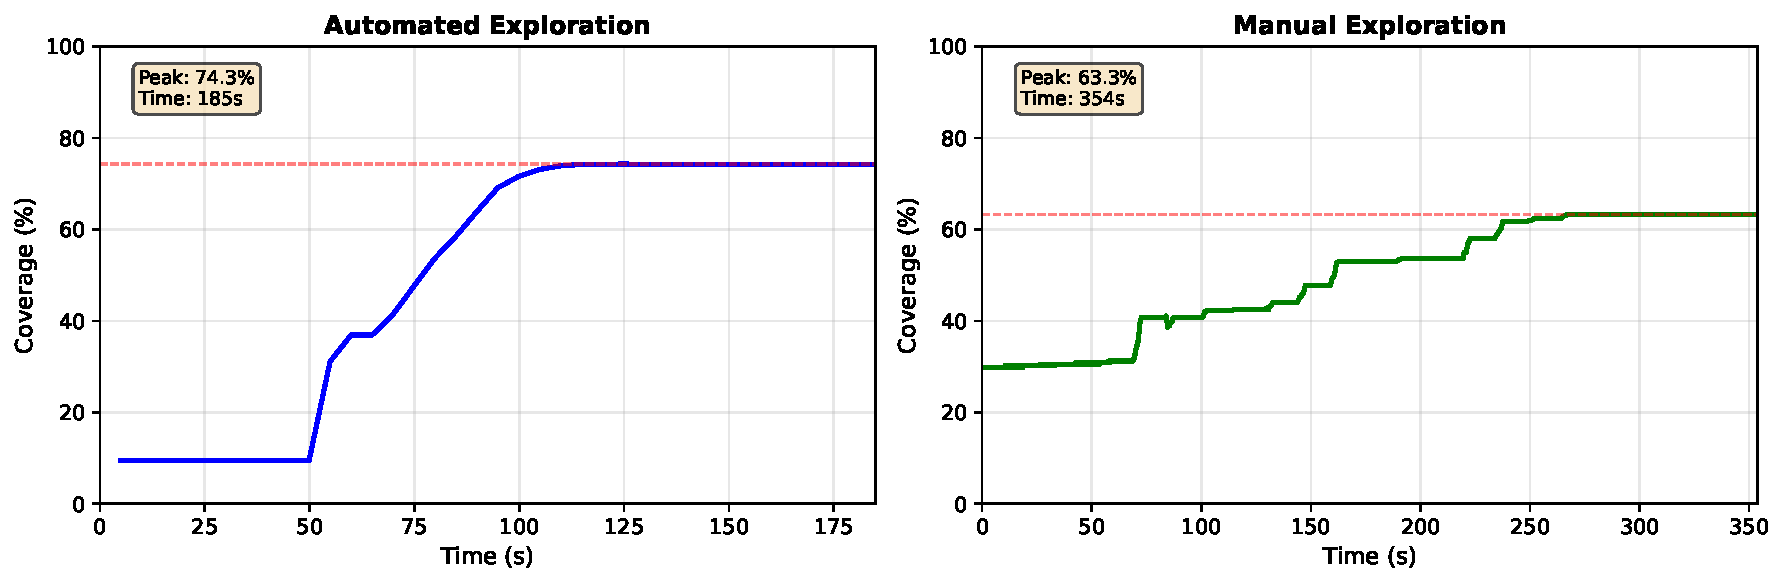
\includegraphics[width=\columnwidth]{figures/coverage_comparison.pdf}
\caption{Coverage over time comparison: Automated exploration (left, blue) achieves 74.3\% coverage in 185s with distinct phases. Manual teleoperation (right, green) reaches only 63.3\% coverage in 354s with irregular progression reflecting human reaction delays.}
\label{fig:coverage}
\end{figure}

\textbf{Coverage Performance:} The automated system achieved 11\% higher peak coverage (74.3\% vs. 63.3\%), demonstrating more systematic exploration compared to human operators.

\textbf{Exploration Speed:} Automated exploration completed in roughly half the time (185s vs. 354s), yielding a 2.24$\times$ efficiency advantage from optimal frontier selection without human reaction delays.

\textbf{Temporal Behavior:} Figure~\ref{fig:coverage} reveals contrasting dynamics. Automated exploration exhibits three phases: (1) initialization (0-50s), (2) rapid exploration (50-100s) with 40\% coverage increase, and (3) saturation (100-185s) plateauing at 74\%. Manual exploration shows irregular progression throughout 354s, reflecting intermittent control inputs and suboptimal path choices.

\subsection{Exploration Progression Analysis}

Figure~\ref{fig:progression} visualizes spatial evolution across three key phases. Initial phase shows limited map knowledge with multiple surrounding frontiers. Mid-exploration reveals hexagonal environment structure with frontiers clustering at room entrances. Final state approaches saturation with all major obstacles mapped; only narrow gaps remain unexplored.

\begin{figure}[h]
\centering
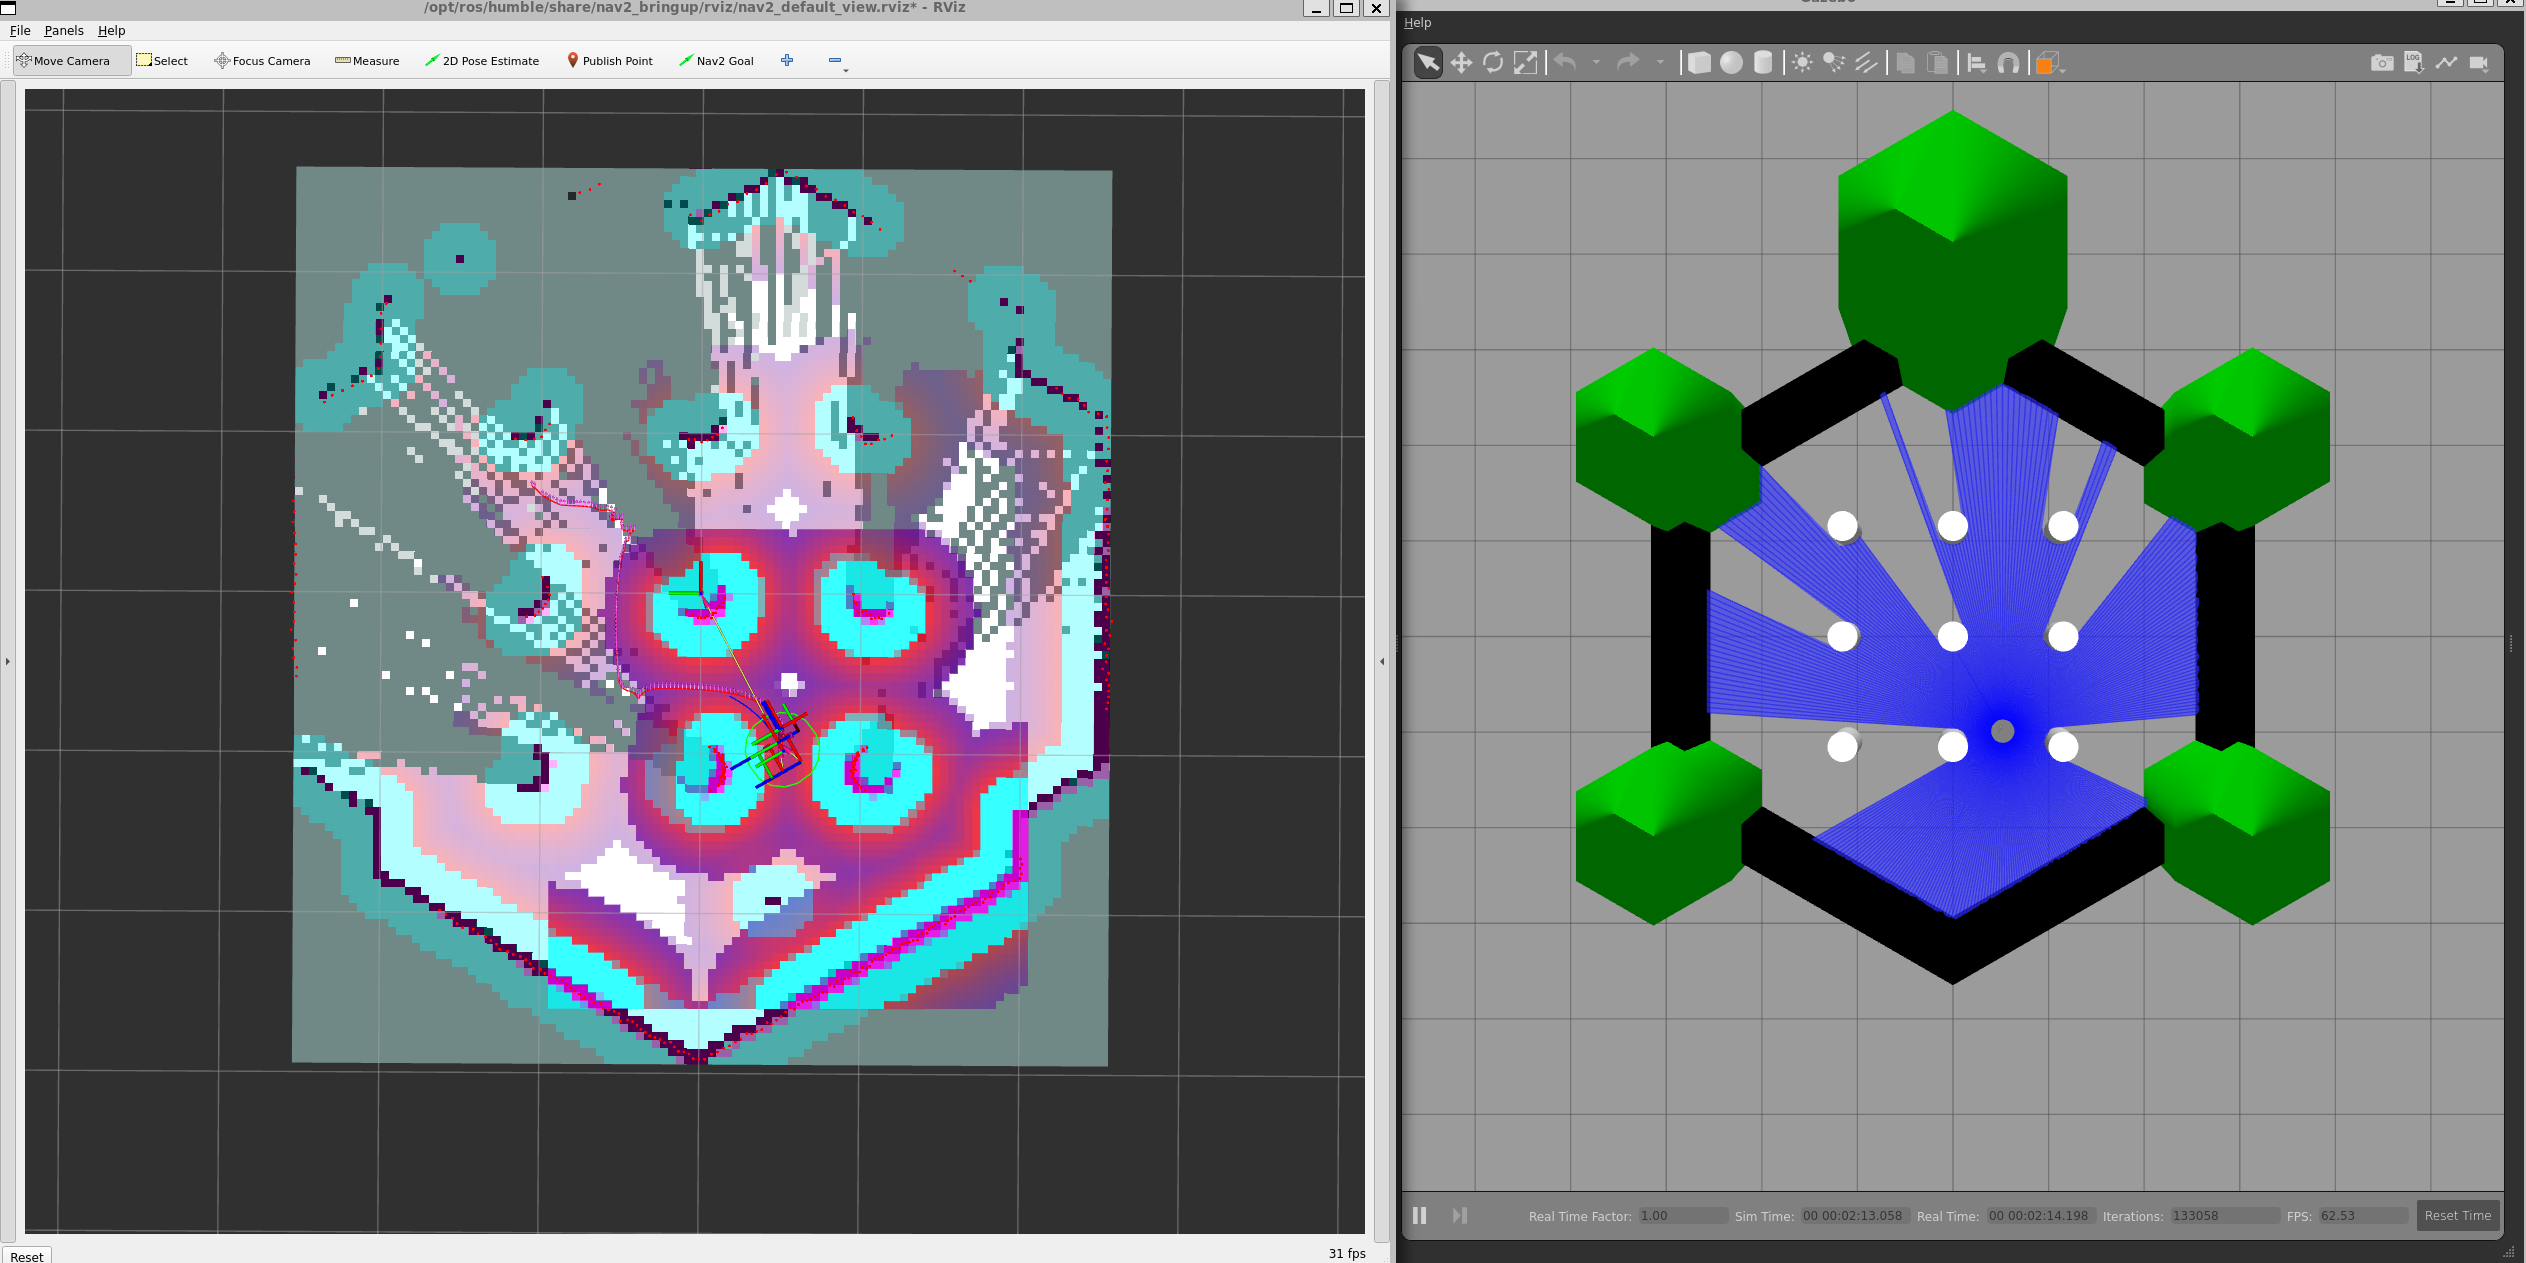
\includegraphics[width=\columnwidth]{figures/Progress_3of6.png}
\caption{Mid-exploration phase showing environment structure emerging. RViz displays occupancy grid (cyan=free, purple=occupied, gray=unknown) with frontier markers (cyan circles) and costmap inflation layers around obstacles.}
\label{fig:progression}
\end{figure}

\subsection{Analysis \& Observations}

\textbf{System Integration:} The 50-second startup delay (visible in Figure~\ref{fig:coverage}) reflects the time required for all ROS2 components to launch, initialize, and establish communication. The initial 10\% coverage represents the immediate sensor field-of-view before autonomous exploration begins. After fixing the explore\_lite bug that initially prevented exploration, the system executes frontier-based navigation correctly.

\textbf{Coverage Saturation:} Neither condition achieved full coverage ($>$95\%). Analysis reveals two causes: (1) narrow corridors ($<$0.75m) rejected by min\_frontier\_size, and (2) costmap inflation blocking paths to remaining frontiers. Reducing the size threshold could improve coverage but risks navigation failures in constrained spaces.

\textbf{Computational Performance:} The low planner\_frequency (0.15 Hz) causes frontier recomputation only every 6.7s, during which the robot may idle. Increasing to 0.5-1.0 Hz could significantly improve exploration rate.

\textbf{Frontier Selection:} The scoring function heavily weights distance (potential\_scale = 3.0) over size (gain\_scale = 1.0), favoring nearby frontiers. While minimizing travel time, this may cause suboptimal global patterns. Information-theoretic approaches could improve long-term efficiency.

\textbf{Map Quality:} Figure~\ref{fig:progression} shows clean, accurate maps with minimal drift. Obstacle boundaries are sharp, and loop closure is robust despite 3+ minutes of operation.

\subsection{Limitations}

Key limitations: (1) single environment testing, (2) simulation only, (3) no systematic parameter sweep, and (4) no failure mode quantification.

\section{Plan Forward}

\subsection{Milestone 2 Objectives}

\textbf{Information-Theoretic Frontier Scoring:} Implement information gain calculation: $\text{Score} = w_1 \cdot \text{IG} + w_2 \cdot (1/\text{Distance}) + w_3 \cdot \text{Uniqueness}$, considering frontier size, expected map expansion, and overlap with other robots.

\textbf{Multi-Robot Task Allocation:} Deploy modified Hungarian algorithm using information-theoretic cost matrix. Solve assignment at 0.5-1 Hz over top-K frontiers per robot with redundant exploration penalties.

\textbf{Multi-Robot Coordination:} Develop two-robot spawn system, integrate multirobot\_map\_merge for confidence-based map merging with ICP, implement distributed architecture.

\textbf{Baseline Optimization:} Optimize planner\_frequency and parameters based on Milestone 1 findings.

\subsection{Final Deliverables \& Risks}

Expected deliverables: (1) complete multi-robot ROS package with information gain scoring, Hungarian task allocation, and map merging; (2) evaluation across three environments demonstrating $\geq$20\% redundancy reduction; (3) ablation studies on key components; (4) scalability testing with 2-4 robots.

\textbf{Risks:} Map merging failure (mitigation: fallback to known poses, confidence thresholds), Hungarian overhead (mitigation: top-K sparsification), bandwidth constraints (mitigation: compressed map deltas).

\section{Conclusion}

We successfully established the baseline single-robot exploration system for our multi-robot project. After debugging critical explore\_lite issues and developing systematic evaluation infrastructure, we achieved 74.3\% coverage with 2.24$\times$ efficiency vs. manual control. This milestone validates our foundation: SLAM-navigation-frontier integration works robustly, automated launch scripts enable repeatable experiments, and metrics collection provides quantitative measurement. Critical findings inform Milestone 2: the 50-second initialization impacts multi-robot synchronization, planner\_frequency (0.15 Hz) needs optimization, and the 74\% ceiling establishes our improvement target. Milestone 2 will implement information gain scoring, Hungarian task allocation, and two-robot coordination to achieve our 20\% redundancy reduction objective.

\section*{Acknowledgments}

We thank the m-explore-ros2 open-source community for providing the foundational codebase and the ROS2 ecosystem for robust robotics middleware.

\bibliographystyle{plainnat}
\begin{thebibliography}{1}

\bibitem{horner2016exploration}
Jiri Horner.
\newblock \href{https://github.com/hrnr/m-explore}{m-explore: Multi-robot exploration package for ROS}.
\newblock GitHub repository, 2016.

\bibitem{yamauchi1997frontier}
Brian Yamauchi.
\newblock A frontier-based approach for autonomous exploration.
\newblock In \emph{Proceedings of the 1997 IEEE International Symposium on Computational Intelligence in Robotics and Automation}, pages 146--151. IEEE, 1997.

\bibitem{burgard2005coordinated}
Wolfram Burgard, Mark Moors, Dieter Fox, Reid Simmons, and Sebastian Thrun.
\newblock Collaborative multi-robot exploration.
\newblock In \emph{Proceedings of the 2000 IEEE International Conference on Robotics and Automation}, volume~1, pages 476--481. IEEE, 2000.

\end{thebibliography}

\end{document}
